\documentclass[12pt]{spieman}

\usepackage{amsmath,amsfonts,amssymb}
\usepackage{graphicx}
\usepackage{setspace}
\usepackage{tocloft}
\usepackage[version=4]{mhchem}
\usepackage{booktabs}
\usepackage{blindtext}


% ---------------------------------------------------------------------------------------
% BEGIN TITLE AND AUTHORS
% ---------------------------------------------------------------------------------------

\title{Improved fluid phantom for accurate relative flow calculations for speckle contrast imaging}

\author[a]{Colin T. Sullender}
\author[a]{Adam Santorelli}
\author[a]{Christopher Smith}
\author[a]{Lisa M. Richards}
\author[a,*]{Andrew K. Dunn}
\affil[a]{Department of Biomedical Engineering, The University of Texas at Austin, Austin, TX, 78712, USA}


% ----------------------------------------------------------------------------------------
% BEGIN DOCUMENT
% ----------------------------------------------------------------------------------------
\renewcommand{\cftdotsep}{\cftnodots}
\cftpagenumbersoff{figure}
\cftpagenumbersoff{table}
\begin{document}
\maketitle


% ----------------------------------------------------------------------------------------
% BEGIN ABSTRACT
% ----------------------------------------------------------------------------------------
\begin{abstract}
Laser speckle contrast imaging (LSCI) is a label-free optical imaging technique that can provide quantitative blood flow data, which can be beneficial during specific neurosurgeries. Microfluidic phantoms are commonly used in the development of LSCI systems as they allow for system characterization and ease of hardware optimization. In this paper, we demonstrate that pressure-driven flow systems can be used to accurately and precisely control flow changes as small as 2\%, in comparison to the commonly used syringe pump systems that have difficulty resolving changes in flow of 5\%. Furthermore, we demonstrate that a multi-exposure speckle imaging (MESI) system is sensitive to small changes in flow and can accurately and repeatably quantify changes in flow as small as 2\%. These results indicate that for the characterization and development of LSCI, or MESI, systems, and to mitigate any concerns with the uncertainty in the actual flow-profile and not the hardware itself, pressure-based flow systems should be used with microfluidic channels.
\end{abstract}

% Include a list of up to six keywords after the abstract
\keywords{multi-exposure speckle imaging, laser speckle contrast imaging, flow measurement, microfluidic, flow system}

% Include email contact information for corresponding author
{\noindent \footnotesize\textbf{*}Andrew K. Dunn \linkable{adunn@utexas.edu}}

\begin{spacing}{2}


% ----------------------------------------------------------------------------------------
% BEGIN INTRODUCTION SECTION
% ----------------------------------------------------------------------------------------
\section{Introduction}
\label{sect:introduction}

Monitoring cerebral blood flow (CBF) is essential during neurosurgery as it provides surgeons with the critical information needed to guide life-saving interventions and is a valuable tool in mitigating post-operative complications \cite{Kirkness.2005}. As such, a clinical system that provides continuous CBF monitoring is highly desired. Laser speckle contrast imaging (LSCI) is a noninvasive, label-free, optical imaging technique based on coherent dynamic light scattering that has been widely implemented for visualizing changes in blood flow \cite{Briers:2001hy,Boas:2010vr}. Requiring only a laser for illumination and a camera for detection, LSCI can produce full-field maps of motion with high spatiotemporal resolution. This has produced great interest in using LSCI for imaging flow in preclinical neuroscience research \cite{Dunn:2001dj,Ayata:2004ba,Bolay:2002jg,Durduran.2004} as well as a broad set of clinical applications spanning the skin \cite{Briers:1996kfa,Choi:2004jn}, retina \cite{Briers.1982,Srienc.2010}, and neurosurgical use \cite{Hecht:2009gu,Parthasarathy:2010gh,Klijn:2012ls}.

Due to its wide adoption, LSCI instrument design and development is an active area of research, and microfluidic studies are commonly used to quantify the visualization of controlled flow changes in modified systems. Typically, studies designed to mimic blood flow involve the use of a flow channel embedded in a polydimethylsiloxane (PDMS) background \cite{Parthasarathy:2008el}, glass capillary tubing \cite{Choi:2004jn}, or clear plastic tubing \cite{Miao:2014}. More complex microfluidic networks have also been fabricated in glass, plastic, and epoxy substrates to represent superficial heterogenous vasculature \cite{Luu.2012}. A scattering solution \cite{Parthasarathy:2008el} or whole blood\cite{Choi:2004jn,Miao:2014} is then flowed through the channel at controlled rates and imaged. For applications in rodent studies, 1 -- 10 mm/s is a commonly selected range of speeds, since this corresponds to the capillary speeds measured in rodents \cite{Tomita:2008do}. This speed is converted to a flow rate using the cross-sectional area of the flow channel, which is used to program the flow control system.

Syringe pumps are the most widely used flow control system in microfluidic studies and are commonly believed to provide a highly-controlled flow output. A review on the subject in 2016 \cite{Richards.2015} found that in the LSCI community, all published microfluidic studies ($>$20) used syringe pumps; this trend has continued to this date with more recent papers continuing to use syringe pump systems for flow control \cite{Zheng:2018ct,Yang.2019}. However, syringe pumps produce oscillations in flow with varying frequency and magnitude due to the physical motion of the motor and from imperfections on the lead screw \cite{Korczyk:2010eu,Li:2014ca}. Syringe pumps have also been shown to have slow responsivity and take a longer time to achieve desired flow rates \cite{Zhou:2011ey}. The trade-off between stability and responsivity makes it difficult to obtain both stable flow and fast flow response with a syringe pump flow control system.

A pressure-driven flow regulation system can overcome the limitations of a syringe pump by eliminating the use of a motor altogether and can provide very stable flow rates \cite{Korczyk:2010eu,Li:2014ca,Zhou:2011ey}. This method involves using compressed air and a pressure regulator to pressurize a reservoir holding the solution, and then applying a controlled pressure to push solution through the microfluidic device at constant flow rates. A feedback loop, with an in-line flow measurement device, can be used to adjust the pressure level to achieve a desired flow rate, which allows the user to request a desired flow rate rather than a pressure level.

One of the primary limitations of LSCI is the difficulty to accurately provide a quantitative assessment of flow, as demonstrated by its weak correlation with in vivo absolute flow velocities in animal studies \cite{Kazmi:2013hp}. Standard LSCI systems use a single camera exposure time, limiting flow sensitivity to a small range. Additionally, several instrumentation factors, namely, illumination variations and noise across different imaging sessions, limits LSCI to intra-patient usage at a single time point and prevents LSCI from providing the quantitative flow data that would be necessary to assist in surgical decision-making. An extension to LSCI called multi-exposure speckle imaging (MESI) has been developed that improves upon many of the shortcomings of LSCI, especially the quantitative accuracy \cite{Parthasarathy:2008el}. MESI has been shown to be reliable for chronic imaging and to have high correlation with in vivo absolute velocities in animal studies \cite{Kazmi:2013hp}, suggesting potential for accurate intra- and inter-patient comparisons. By using multiple camera exposure times spanning multiple decades and a more robust mathematical model to estimate flow velocity, the MESI technique has higher accuracy and sensitivity compared to LSCI \cite{Parthasarathy:2008el}.

In this paper, we address two primary objectives: first, we quantify the uncertainty associated with both a syringe pump and a pressure regularized flow system. By understanding the associated uncertainty with each system, we can provide insight on the experimental design for a microfluidic study that aims to assess the hardware performance of an optical system, without fear that performance can be compromised due to flow-related noise. Quantifying this error allows us to accurately determine the true sensitivity to relative flow changes of a MESI system. Secondly, we demonstrate that a MESI system can resolve very small changes in relative flow, as small as 2\%. The ability for MESI to resolve such small changes in relative flow, which are smaller than the combined uncertainty of the syringe pump system, indicate that to properly assess the performance of novel hardware for a LSCI or MESI system, a pressure-driven flow system should be used.

The remainder of the paper can be summarized as follows: Section \ref{sect:methods} describes the microfluidic phantom fabrication and the different experimental tests to assess the uncertainty with the syringe pump and pressure regulated systems, the instrumentation for the MESI system, and the mathematical formulation necessary to calculate relative flow from the data collected with the MESI system. Results from these experimental protocols, namely the uncertainty analysis and the MESI flow calculations, are presented in Section \ref{sect:results}. Lastly, the paper findings and contributions are summarized in Section \ref{sect:discussion}.


% ----------------------------------------------------------------------------------------
% BEGIN METHODS SECTION
% ----------------------------------------------------------------------------------------
\section{Methods}
\label{sect:methods}

\subsection{Microfluidic Phantom Fabrication}
The microfluidic flow phantom was cast using PDMS (Sylgard 184™, Dow Corning) with 1.8 mg titanium dioxide (\ce{TiO2}) per gram of PDMS added to generate a scattering background that mimicked tissue optical properties ($\mu_s' = 8$ cm$^{-1}$) \cite{Parthasarathy:2008el,Yaroslavsky:2002tg}. The PDMS \ce{TiO2} mixture was vigorously mixed for 15 minutes to ensure even distribution of the \ce{TiO2} in the phantom. Centrifugation (3000 g relative centrifugal force, 10 minutes) was then performed to de-gas the sample and remove any \ce{TiO2} clumps.

A machined aluminum mold was used to cast the microchannel, shown in Fig.~\ref{fig:microfluidic}a. The extrusion is 460 $\mu$m $\times$ 460 $\mu$m $\times$ 25 mm, which formed three walls of the microfluidic channel. A square cross-section (1:1 aspect ratio) was desired to match the aspect ratio of the circular cross-section vascular geometries in vivo. The PDMS \ce{TiO2} mixture was carefully poured on top of the mold within a polystyrene petri dish and placed in a vacuum chamber to remove air bubbles introduced during pouring. The PDMS was then cured at 70 $^\circ$C for 45 -- 60 minutes, allowed to cool, and detached from the mold. The microchannel side of the phantom was oxygen plasma bonded to a glass slide to seal the channel. Inlet and outlet ports were attached using 23G blunt tip needles fitted partially inside the phantom, which were epoxied in place for an air-tight seal. Tygon® microbore tubing (0.02$''$ inner diameter, Cole Parmer Instrument Company, LLC.) was used to connect to the blunt tip ports as inlet and outlet tubing. The inlet tubing was connected to the flow sensor and the flow control system using fluidic fittings with FEP tubing (IDEX Health and Science, LLC.). The outlet tubing drained into a vial, with the tubing end submerged in solution. A photograph of the finished phantom is shown in Fig.~\ref{fig:microfluidic}b, where the channel is visible inside the white PDMS and the glass slide seals the surface.

% Figure 1 - Microfluidic Flow Phantom
\begin{figure}
    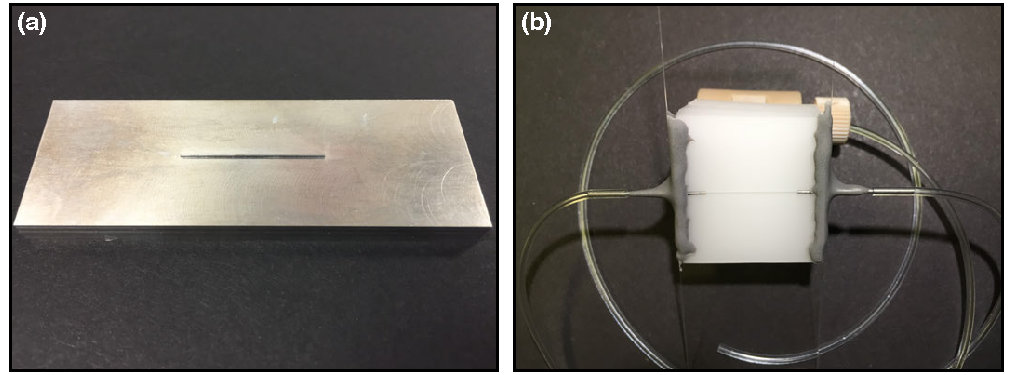
\includegraphics[width=\textwidth]{Figure1.pdf}
    \caption {
        (a) Photograph of the machined aluminum mold with a 460 $\mu$m $\times$ 460 $\mu$m $\times$ 25 mm, extrusion used to cast the PDMS during fabrication of the microfluidic flow phantom. (b) Photograph of the finished microfluidic flow phantom, showing PDMS bonded to a glass slide, with inlet and outlet ports secured using epoxy. Tubing was secured to the ports and connected with the rest of the system using fluidic fittings.
    }
    \label{fig:microfluidic}
\end{figure}

A colloidal mixture of suspended 1 $\mu$m diameter polystyrene microspheres (10\% w/w, 5100A, Thermo Fisher Scientific, Inc.) in ultra-filtered de-ionized (UFDI) water was used as a blood-mimicking solution. Based on Ref. \cite[]{Roggan:1999bz}, the reduced scattering coefficient ($\mu_s'$) of whole blood with hematocrit = 0.5 is approximately 20 cm$^{-1}$. By using a 7\% by volume mixture of the polystyrene microsphere solution and UFDI water (for example, a 10 mL batch of the blood mimicking solution would be made up of by 0.7 mL of the 5100A solution and 9.3 mL UFDI water) we are able to achieve a calculated $\mu_s'$ of 19.8 cm$^{-1}$. However, we note that the anisotropy of the microspheres in our solution is different that that of whole blood ($g = 0.92$ compared to $g = 0.98$). The blood-mimicking solution was preferred over whole blood for several reasons, namely: cleaning and safety, ease of acquisition, and because the flow sensor was factory-calibrated for deionized water flow. Since the concentration of microspheres was very low (0.7\% by weight in the final suspension), the water calibration of the flow sensor remained valid. The solution of microspheres was freshly mixed before each experiment to reduce aggregation of particles in the dilution. Once mixed, the solution was sonicated (10 minutes) to fully suspend the particles and then de-gassed under vacuum to eliminate air bubbles.


\subsection{Microfluidic Flow System Instrumentation}

To assess the performance of the syringe pump and pressure-regulated flow systems, and to quantify the uncertainty of each system, it is necessary to know the true flow rate of the blood-mimicking solution through the microfluidic channel. A mass flow sensor (FLU-L, 0 -- 1 mL/min, Fluigent, Inc.) was placed inline between the flow control system and the phantom inlet tubing, as shown in Fig.~\ref{fig:system}a. The sensor was connected to a flow reader (Flow Board, FLB, Fluigent, Inc.) to digitize the sensor output and the MAESFLO software (Fluigent, Inc.) recorded the absolute flow rate.

The syringe pump system (74905-04, Cole-Parmer Instrument Company, LLC.) was connected to the flow sensor, as shown in Fig.~\ref{fig:system}b, and a 10 mL plastic syringe (BD \#302149) was filled with blood-mimicking solution. The syringe pump was programmed to run the desired flow profile, using the inner diameter of the syringe to ensure correct flow rate output (10 mL = 14.5 mm). It should be noted that a 3 mL syringe was also tested, however its performance was significantly worse than the 10 mL syringe and, in some cases, could not resolve the desired flow profiles.

The pressure-regulated flow system used a pressure controller base unit (MFCS-EZ with 69 mbar channel, Fluigent, Inc.), powered by a house air line regulated to maintain 500 mbar of pressure, as shown in Fig.~\ref{fig:system}c. This controller outputted regulated air flow (up to 69 mbar) to a 15 mL pressurized reservoir (Fluiwell-1C, Fluigent, Inc.) filled with blood-mimicking solution. Prior to running the desired flow program, a calibration was performed that accounted for the resistance from the tubing, microfluidic channel, and hydrostatic pressure. The pressure control system used built-in software (MAESFLO) to provide feedback from the inline flow sensor to regulate the pressure to achieve the desired flow rate.


\subsection{Microfluidic Flow System Assessment}

Two stepped flow profile experiments were conducted to assess each flow system. First, a 3-step flow profile was used to determine the uncertainty of each flow control system. The experiment lasted 240 seconds, beginning with 30 seconds of no flow (0 mm/s) followed by one full minute at each flow speed (2.4, 3.6, and 4.8 mm/s) before concluding with an additional 30 seconds of no flow. The experiment was repeated three times on each system. The second flow profile experiment consisted of a 13-step flow profile. The flow speed was once again varied from 2.4 to 4.8 mm/s, however in smaller 0.2 mm/s increments. As with the first experiment, the flow profile begins and ends with 30 seconds of no flow, with one full minute at each programmed flow speed (840 seconds total duration). The second experiment was also repeated three times on each flow control system.

To quantify and compare each system, we calculated the total combined uncertainty in accordance with National Institute of Standards and Technology (NIST) guidelines \cite{Taylor.199438,NIST:2002}. Three main sources of uncertainty were identified for inclusion in the uncertainty budget: repeatability, reproducibility, and measurement bias. Standard uncertainties were calculated for each flow step using 55 seconds of data, allowing for 5 seconds of transition from the previous flow state. All values were expressed as percentages relative to their respective means.

The uncertainty in repeatability, which is a measure of within-run variance, was defined as:
%
% Equation 1 - Uncertainty in Repeatability
\begin{equation}
    \label{eq:u_repeat}
    u_\textnormal{repeat} = 100 \times \frac{s_p}{\bar{x}}
\end{equation}

\noindent where $s_p^2$ is the pooled variance across the three trials at each flow speed and $\bar{x}$ is the mean value of the measured flow speed across all trials.

The uncertainty in reproducibility, which is a measure of between-run variance, was defined as:
%
% Equation 2 - Uncertainty in Reproducibility
\begin{equation}
    \label{eq:u_reproduce}
    u_\textnormal{reproduce} = 100 \times \frac{s}{\bar{x}}
\end{equation}

\noindent where $s^2$ is the variance in the mean flow speed across all three trials and $\bar{x}$ is the mean value of the measured flow speed across all trials.

Finally, the uncertainty in measurement bias, was defined as:
%
% Equation 3 - Uncertainty in Bias
\begin{equation}
    \label{eq:u_bias}
    u_\textnormal{bias} = 100 \times \left| \frac{\bar{x} - x_{ref}}{x_{ref}} \right|
\end{equation}

\noindent where $\bar{x}$ is the mean value of the measured flow speed across all trials and $x_{ref}$ is the programmed flow speed (2.4, 3.6, or 4.8 mm/s) at each step.

The total combined standard uncertainty ($u_c$) was then calculated using the root sum of squares of the individual uncertainty components and reported as the expanded uncertainty ($U=ku_c$) with a $k=2$ coverage factor corresponding to a level of confidence of approximately 95\%.


\subsection{MESI Instrumentation}

A schematic of the imaging setup is shown in Fig.~\ref{fig:system}a. MESI was performed \cite{Parthasarathy:2008el} using a wavelength-stabilized 785 nm laser diode (LD785-SEV300, Thorlabs, Inc.) mounted in a temperature-controlled housing (TCLDM9, Thorlabs, Inc.) and collimated using an aspheric lens (C280TMD-B, Thorlabs, Inc.). The operating current on the laser diode controller (LDC205C, Thorlabs, Inc.) was fixed at 380 mA (300 mW) and the target temperature set to 25 $^\circ$C on the temperature controller (TED200C, Thorlabs, Inc.). The collimated laser light was passed through a free-space optical isolator (Electro-Optics Technology, Inc.) to minimize back reflections that interfere with single frequency performance. Because the external volume holographic grating of the stabilized laser diode produces a dark spot in the far field, the laser was coupled into a single-mode patch cable (P3-780A-FC-2, Thorlabs, Inc.) to obtain a Gaussian beam. The fiber output was re-collimated (F230APC-780, Thorlabs, Inc.), intensity modulated with an acousto-optic modulator (AOM, 3100-125; RF Driver 1110AF-AIFO-1.0, Gooch \& Housego, Ltd.), and relayed to obliquely illuminate the sample.

A pair of consumer camera lenses were used to image the scattered light (AF Nikkor 50 mm $f$/1.8D + AF Micro-Nikkor 105 mm $f$/2.8D, Nikon Corp.) with 2.1$\times$ magnification through a bandpass filter (785$\pm$31 nm, 87-773, Edmund Optics Inc.) to a CMOS camera (acA1920-155um, 1920 $\times$ 1200 pixels, Basler AG). Only a subset of the overall sensor array was used (1000 $\times$ 750 pixels), resulting in a field-of-view of 2.9 $\times$ 2.2 mm. The camera exposures were temporally synchronized with the modulated laser pulses. Fifteen different camera exposures ranging between 50 $\mu$s and 80 ms were recorded for each complete MESI frame, resulting in an effective acquisition rate of $\sim$2.5 frames-per-second (fps). The total amount of light used to capture each exposure was held constant with the AOM in order to minimize the effects of shot noise \cite{Parthasarathy:2008el}. The entire acquisition was controlled using custom software written in C++ along with a multifunction I/O device (USB-6363, National Instruments Corp.) for the generation of camera exposure trigger signals and AOM modulation voltages.

% Figure 2 - System Schematic
\begin{figure}
    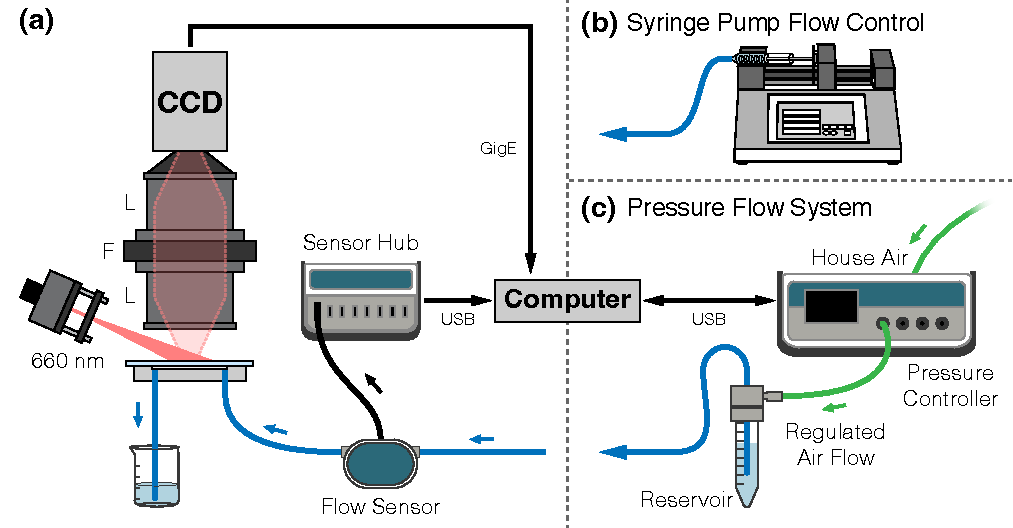
\includegraphics[width=\textwidth]{Figure2.pdf}
    \caption {
        (a) Optical system schematic for microfluidic flow assessment. A commercial flow sensor was placed in series with the inlet tubing for the microfluidic flow phantom to obtain real-time absolute flow measurements. Flow was programmatically controlled using either a (b) syringe pump or (c) pressure-regulated flow system. The software for the pressure flow system used a feedback loop between the flow sensor readings and the pressure controller to regulate air pressure.
    }
    \label{fig:system}
\end{figure}


\subsection{MESI Microfluidic Flow Measurements}

A stepped flow profile experiment was conducted using the pressure-regulated flow system to assess the performance of MESI. The flow profile consisted of 19 steps spanning 1 -- 10 mm/s in 0.5 mm/s increments. Each speed was maintained for two minutes with a total duration of 40 minutes, including brief periods of no flow (0 mm/s) at the beginning and end of the profile. MESI measurements were acquired continuously throughout the experiment at the maximum acquisition rate of the system ($\sim$2.5 fps). Because the flow sensor software used a separate clock than the MESI acquisition, the datasets were synchronized during post-processing using the initial rise of the first flow step. The experiment was repeated a total of four times across two days.

Raw intensity images were converted to speckle contrast images ($K = \sigma_{s} / {\langle{I}\rangle}$) using a 7$\times$7-pixel sliding window. The average speckle contrast of each frame was then calculated within a region centered in the microfluidic channel and used to estimate the correlation time ($\tau_c$) of the speckle autocorrelation function, which is considered a more quantitative measure of flow \cite{Briers:1996kfa}. The averaged speckle contrast values were fitted to the multi-exposure speckle visibility equation \cite{Parthasarathy:2008el} using all fifteen exposure times to obtain $\tau_c$:
%
% Equation 1 - MESI Equation
\begin{equation}
    \label{eq:mesi}
    K^2(T,\tau_c) =
        \beta\rho^2\frac{e^{-2x} - 1 + 2x}{2x^2} +
        4\beta\rho(1 - \rho)\frac{e^{-x} - 1 + x}{x^2} +
        \nu
\end{equation}

\noindent where $T$ is the camera exposure time, $x=T/\tau_c$, $\rho$ is the fraction of light that is dynamically scattered, $\beta$ is a normalization factor that accounts for speckle sampling, and $\nu$ represents exposure-independent instrument noise and nonergodic variances. $\beta$ was held constant at all timepoints by performing an initial fit to Eq. 3 using the median speckle contrast value at each exposure across the entire multi-exposure dataset. All fitting was performed with the Levenberg-Marquardt nonlinear least squares algorithm \cite{Lourakis:J2fCMU5i} using a custom program written in MATLAB (R2021a, MathWorks, Inc.). The resulting $\tau_c$ estimates were smoothed temporally using a central moving average filter ($k=5$).

Because $\tau_c$ is inversely related to the speed of moving scatterers in the sample \cite{Bonner:1981hg}, the inverse correlation time ($ICT = 1/\tau_c$) is commonly used to visualize measurements. In order to directly compare the MESI measurements with the flow sensor, the relative flow was calculated using the average value of the 1 mm/s step as the baseline ($rICT = ICT/ICT_\textnormal{1mm/s}$). The average value of each flow step was calculated using 115 seconds of data, allowing for 5 seconds of transition from the previous step.


% ----------------------------------------------------------------------------------------
% BEGIN RESULTS SECTION
% ----------------------------------------------------------------------------------------
\section{Results}
\label{sect:results}

\subsection{Microfluidic Flow System Assessment}

A comparison between the measured flow speeds of the syringe pump and the pressure-regulated flow system is shown in Fig.~\ref{fig:syringe_vs_pressure}. From these plots, we observe that the pressure-regulated system outperforms the syringe pump system by accurately and steadily reaching the programmed flow speeds in both experiments. While both systems quickly responded to the desired flow changes (Fig.~\ref{fig:syringe_vs_pressure}a), the syringe pump system suffered from accuracy and stability issues compared to the pressure-regulated system. Furthermore, the small flow step experiment (Fig.~\ref{fig:syringe_vs_pressure}b) demonstrated that the syringe pump system cannot reliably produce finer flow changes as seen by the loss of the stair-stepped flow pattern.

% Figure 3 - Syringe Pump vs. Pressure System
\begin{figure}
    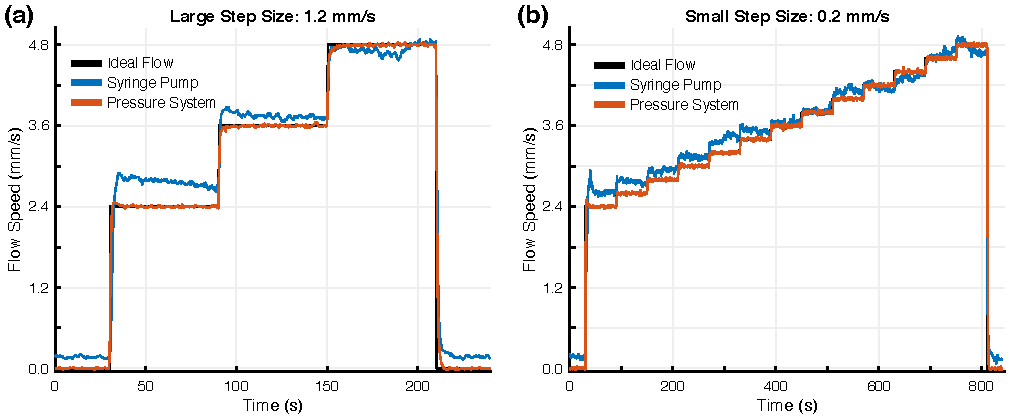
\includegraphics[width=\textwidth]{Figure3.pdf}
    \caption {
        Flow profiles for the syringe pump (blue) and pressure-regulated (red) flow systems compared to the ideal programmed flow (black) for one run of the (a) 3-step and (b) 13-step experiments. The microfluidic flow speed varied between 2.4 to 4.8 mm/s in 1.2 mm/s and 0.2 mm/s steps for the 3- and 13-step experiments, respectively.
    }
    \label{fig:syringe_vs_pressure}
\end{figure}

Table~\ref{tab:uncertainty_standard} shows a comparison of the standard uncertainties for repeatability ($u_\textnormal{repeat}$), reproducibility ($u_\textnormal{reproduce}$), and bias ($u_\textnormal{bias}$) for each system at the flow speeds tested in the 3-step experiment. These results confirm the observations from Fig.~\ref{fig:syringe_vs_pressure} that the pressure-regulated flow system is more stable, repeatable, and accurate at all the tested flow speeds. The combined and expanded uncertainties for both systems are presented in Table~\ref{tab:uncertainty_combined}. These results provide evidence of the superiority of the pressure-regulated flow system, particularly when attempting to produce small flow changes. With the syringe pump system, it would be impossible to reliably separate changes in relative flow of 20\% from flow system noise at the 2.4 mm/s flow speed. This magnitude of uncertainty in flow generation would make it difficult to assess an optical system’s ability to detect small changes in flow. This limitation is visually represented in Fig.~\ref{fig:syringe_vs_pressure}b, where the syringe pump fails to resolve the finer 0.2 mm/s flow changes. Using the pressure-regulated flow system, we can confidently design experiments with relative flow changes of only 1.5\% and be certain that the resulting optical system measurements are not due to flow system noise. Furthermore, this would allow for the assessment of improvements to optical system performance at this scale.

\begin{table}
    \caption {
        Standard uncertainties for repeatability, reproducibility, and bias by flow speeds for the syringe pump and pressure-regulated flow systems.
    }
    \label{tab:uncertainty_standard}
    \centering
    \begin{tabular}{rccccccccc}
        \addlinespace
        \toprule
            &
            \multicolumn{3}{c}{$\boldsymbol{u_\textbf{repeat}}$ (\%)}       & 
            \multicolumn{3}{c}{$\boldsymbol{u_\textbf{reproduce}}$ (\%)}    & 
            \multicolumn{3}{c}{$\boldsymbol{u_\textbf{bias}}$ (\%)}         \\
            \cmidrule(lr){2-4}
            \cmidrule(lr){5-7}
            \cmidrule(lr){8-10}
        \textbf{Flow Speed (mm/s)} & 2.4    & 3.6   & 4.8   & 2.4   & 3.6   & 4.8   & 2.4   & 3.6   & 4.8   \\
        \midrule
        \textbf{Syringe Pump}      & 1.31   & 0.90  & 1.86  & 4.01  & 2.15  & 1.07  & 10.3  & 1.80  & 2.55  \\
        \textbf{Pressure System}   & 0.55   & 0.45  & 0.39  & 0.002 & 0.009 & 0.003 & 0.03  & 0.07  & 0.03  \\
        \bottomrule
    \end{tabular}
\end{table}

\begin{table}
    \caption {
        Combined and expanded uncertainties (with $k=2$ coverage) by flow speeds for the syringe pump and pressure-regulated flow systems.
    }
    \label{tab:uncertainty_combined}
    \centering
    \begin{tabular}{rcccccc}
        \addlinespace
        \toprule
            &
            \multicolumn{3}{c}{$\boldsymbol{u_c}$ (\%)}     &
            \multicolumn{3}{c}{$\boldsymbol{U}$ (\%)}       \\
            \cmidrule(lr){2-4}
            \cmidrule(lr){5-7}
        \textbf{Flow Speed (mm/s)} & 2.4    & 3.6   & 4.8   & 2.4   & 3.6   & 4.8   \\
        \midrule
        \textbf{Syringe Pump}      & 11.1   & 2.94  & 3.34  & 22.2  & 5.89  & 6.68  \\
        \textbf{Pressure System}   & 0.56   & 0.45  & 0.39  & 1.11  & 0.91  & 0.77  \\
        \bottomrule
    \end{tabular}
\end{table}


\subsection{MESI Microfluidic Flow Measurements}

The MESI microfluidic flow measurements using only the pressure-regulated flow system are shown in Fig.~\ref{fig:mesi_flow}. The relative flow measured by MESI ($rICT$) is plotted alongside the relative flow sensor measurements from a single trial in Fig.~\ref{fig:mesi_flow}a. Both metrics were calculated using the average of the first flow step (1 mm/s) as the baseline. Data for each flow step were pooled and averaged across all four trials to assess the overall performance of MESI as seen in Fig.~\ref{fig:mesi_flow}b. The coefficient of determination ($R^2$) and concordance correlation coefficient ($\rho_c$) \cite{Lin.1989} were 0.988 and 0.994, respectively, indicating strong agreement between the MESI $rICT$ and the flow sensor measurements. The absolute MESI $ICT$ measurements are also plotted on Fig.~\ref{fig:mesi_flow}b and exhibit the same linearity with microfluidic flow speed.

% Figure 4 - MESI Flow Measurements
\begin{figure}
    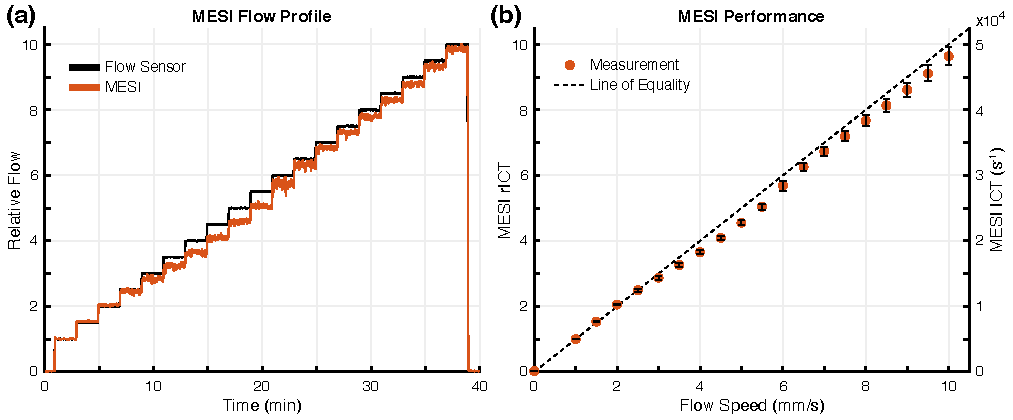
\includegraphics[width=\textwidth]{Figure4.pdf}
    \caption {
        (a) Relative flow profiles for the flow sensor (black) and MESI (red) for one trial, both normalized to the average of the first flow step (1 mm/s). (b) Performance of MESI flow estimates (relative and absolute) compared to measured microfluidic flow speed aggregated across all four trials (mean $\pm$ sd). The dashed line denotes the line of equality indicative of a 1:1 relationship.
    }
    \label{fig:mesi_flow}
\end{figure}

Fig.~\ref{fig:mesi_error} presents the percent error for the MESI measurements at each flow step aggregated across all four trials. The absolute error was below 5\% except for flow speeds between 3.5 to 6 mm/s, where it almost doubled in value.

% Figure 5 - MESI Error
\begin{figure}
    \centering
    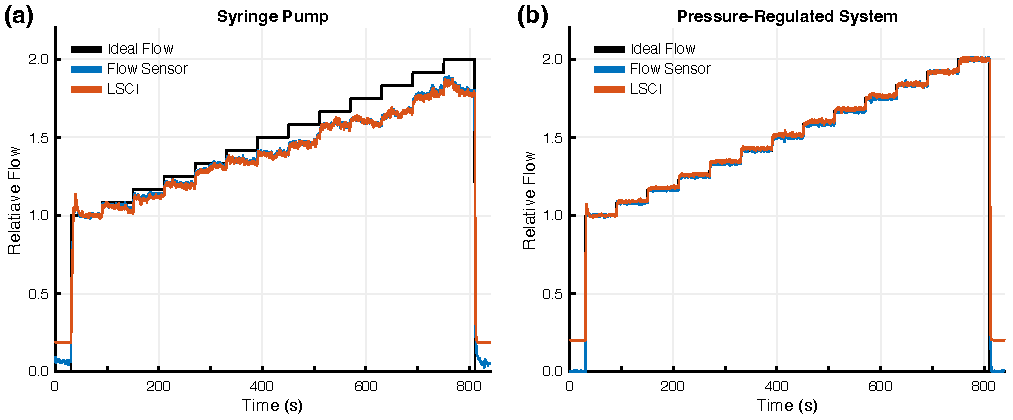
\includegraphics[width=0.5\textwidth]{Figure5.pdf}
    \caption {
        Percent error for MESI $rICT$ measurements at each flow step relative to the flow sensor measurements.  Data aggregated by flow step across all four trials.
    }
    \label{fig:mesi_error}
\end{figure}


% ----------------------------------------------------------------------------------------
% BEGIN DISCUSSION SECTION
% ----------------------------------------------------------------------------------------
\section{Discussion}
\label{sect:discussion}

\blindtext


% ----------------------------------------------------------------------------------------
% BEGIN CONCLUSION SECTION
% ----------------------------------------------------------------------------------------
\section{Conclusion}
\label{sect:conclusion}

This paper demonstrates that pressure-regulated flow systems should be used instead of syringe pumps when assessing the performance of optical imaging systems using microfluidics. We determine that the uncertainty in flow generation with a pressure-regulated flow system is considerably less than that of a syringe pump system across a range of physiologically-relevant flow speeds. Furthermore, we demonstrate that MESI can be used to detect changes in relative flow as small as 5\%. Given the large uncertainties associated with syringe pump systems, it would be impossible to determine that such a measurement arose from an actual flow change rather than random or systematic error. These results indicate that it is necessary to use a pressure-regulated flow system in order to properly assess the performance of a MESI system or when characterizing hardware changes to such a system.


% ----------------------------------------------------------------------------------------
% BEGIN DISCLOSURES AND ACKNOWLEDGEMENTS
% ----------------------------------------------------------------------------------------
\subsection*{Disclosures}
A.K.D. holds equity in Dynamic Light, Inc. The authors declare no other conflicts of interest.

\subsection*{Author Contributions}
C.T.S. and L.M.R. constructed the imaging system, conceived the experiments, and acquired the data. C.T.S., A.S., and L.M.R. analyzed the results and wrote the manuscript. A.K.D. supervised the project. All authors contributed to the manuscript revisions.

\subsection*{Acknowledgments}
This study was supported by the National Institutes of Health (Nos. ?)

\subsection* {Data, Materials, and Code Availability} 
The code and data that support the findings of this study are available from the corresponding author, A.K.D., upon reasonable request.


% ----------------------------------------------------------------------------------------
% BEGIN BIBLIOGRAPHY
% ----------------------------------------------------------------------------------------
\bibliography{bibliography}
\bibliographystyle{spiejour}


% ----------------------------------------------------------------------------------------
% AUTHOR BIOGRAPHIES
% ----------------------------------------------------------------------------------------
\vspace{1ex}
\vspace{2ex}\noindent\textbf{First Author} is an assistant professor at the University of Optical Engineering. He received his BS and MS degrees in physics from the University of Optics in 1985 and 1987, respectively, and his PhD degree in optics from the Institute of Technology in 1991.  He is the author of more than 50 journal papers and has written three book chapters. His current research interests include optical interconnects, holography, and optoelectronic systems. He is a member of SPIE.

\vspace{1ex}
\noindent Biographies and photographs of the other authors are not available.


% ----------------------------------------------------------------------------------------
% FIGURE AND TABLE LISTS
% ----------------------------------------------------------------------------------------
\listoffigures
\listoftables


% ----------------------------------------------------------------------------------------
% END
% ----------------------------------------------------------------------------------------
\end{spacing}
\end{document}
